
\documentclass{beamer}

\usepackage{graphicx}
\usepackage[light]{FiraSans}
\usepackage[british]{datetime2}
\usetheme{default}
\setbeamertemplate{navigation symbols}{} % No navigation symbols
\definecolor{ntnu}{cmyk}{100,75,0,5}
\setbeamercolor{alerted text}{fg=ntnu}
\setbeamercolor{frame title}{fg=ntnu}
\setbeamercolor{title}{fg=ntnu}
\setbeamercolor{subtitle}{fg=ntnu}
\setbeamercovered{transparent}

\setbeamertemplate{itemize item}{\color{white}$\bullet$} % Comment this line for default bullet points (triangles)

\setbeamertemplate{footline}
{
	\begin{center}
	\begin{tabular}{ccccc|c}
	\raisebox{-0.3cm}{
\includegraphics[width=2cm, keepaspectratio]{logo_ntnu_u-slagord.pdf}} &
	\insertshortauthor & 
	\insertshorttitle &
	\insertdate &
	\insertsection
	\hspace{2cm} &
	\insertframenumber
	\end{tabular}
	\end{center}
}

\makeatletter
\makeatother

%----------------------------------------------------------------------------------------
%	TITLE PAGE
%----------------------------------------------------------------------------------------

\title[POL2012]{Evolutionary economics \& Modern political economy}

\subtitle{}

\author[Wishman]{Marius Swane Wishman} 
\date{\today} 
\institute{ISS}

\begin{document}

\begin{frame}[plain]
\titlepage 
\centering

\includegraphics[width=5cm]{logo_ntnu_u-slagord.pdf} 
\end{frame}

%----------------------------------------------------------------------------------------
%	Beginning of document
%----------------------------------------------------------------------------------------

\section{The other Canon} 

\begin{frame}
\frametitle{The other Canon}

\begin{itemize}
	\item Other canon, evolutionary economics experienced-based economics,
		historical economics, reality economics etc.
	\item A response to the gap between the classical theories and the
		actual policy pursued by their proponents\pause
	\item Biology not physics \pause
	\item Induction not deduction \pause
	\item Production not exchange or distribution
\end{itemize}
	
\end{frame}

\section{Development through stages}

\begin{frame}{National economics}

\begin{itemize}
	\item Friedrich List (1789-1846)
	\item A word of caution! \pause
	\item Right, not more or or less
	\item Development through stages % HUGE political influence,
		% theoretically it took a while to catch on. Free trade,
		% protection, free trade. Temporary sacrifice likened to education
\end{itemize}	

\end{frame}

\section{Joseph Schumpeter 1883-1950}

\begin{frame}{Creative Destruction}

\begin{figure}
    \centering
    %  Builds on Marx, List and others	
    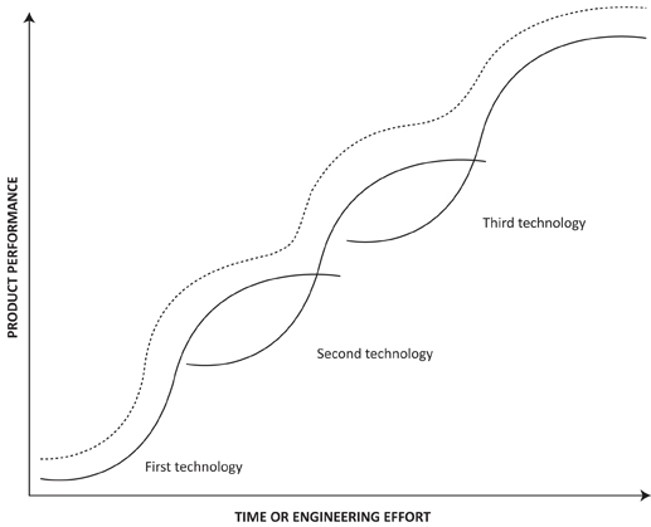
\includegraphics[width=0.9\textwidth]{../img/CreativeDestruction.jpg}
\end{figure}{}

\end{frame}

\begin{frame}

	\begin{itemize}
		\item The road through Galbraith to socialism \pause
		% Innovation is the key to progress
		% Capitalism unleashed the beast, but will ultimately tame it to
			% its own detriment
		\item The legacy of Schumpeter
		% Innovation is the key to progress! ... And is cool!
	\end{itemize}

\end{frame}{}

\begin{frame}{The legacy of Schumpeter}

\begin{figure}[htpb]
	\centering
	
\includegraphics[width=0.9\linewidth]{../img/yayscience.png}
	\caption{Science is cool!}%
\end{figure}	

\end{frame}

\begin{frame}{But is it that simple?}

	\centering
	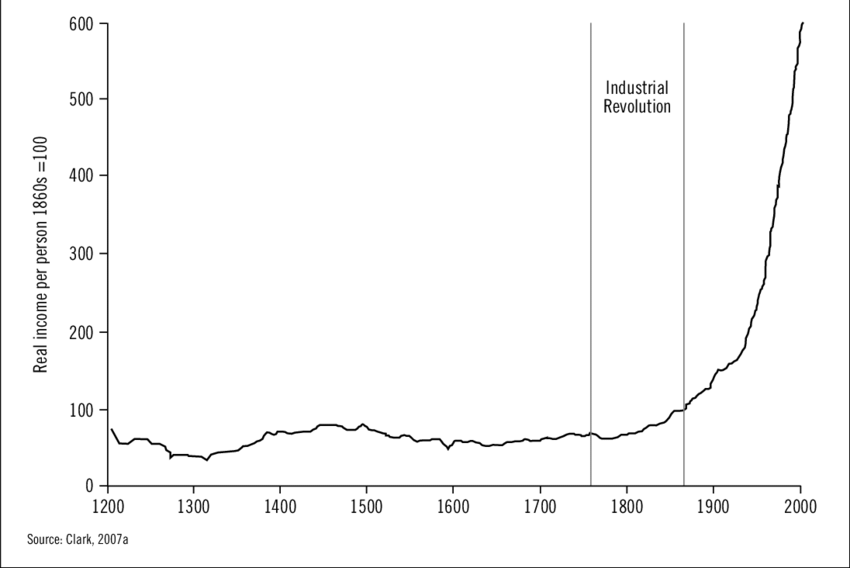
\includegraphics[width=\textwidth]{../img/realincome.png} 
	% Economic growth? Yes, but progress?
    	% Two stories, Socialist or QEA

\end{frame}

\section{Erik Reinert 1949-}

\begin{frame}{Quality of economic activity}

	% Reiterates and synthesises the "canon"
	% Production! Sequencing! Pulling up the ladder!
	% "Adds" synergies, activities dependent on human capital (last figure)
	% Increasing vs decreasing returns
		% Production expands -> prod.cost per unit falls
			% Economies of scale
		% As opposed to "regular labor" and agriculture
	\begin{figure}[htpb]
		\centering
		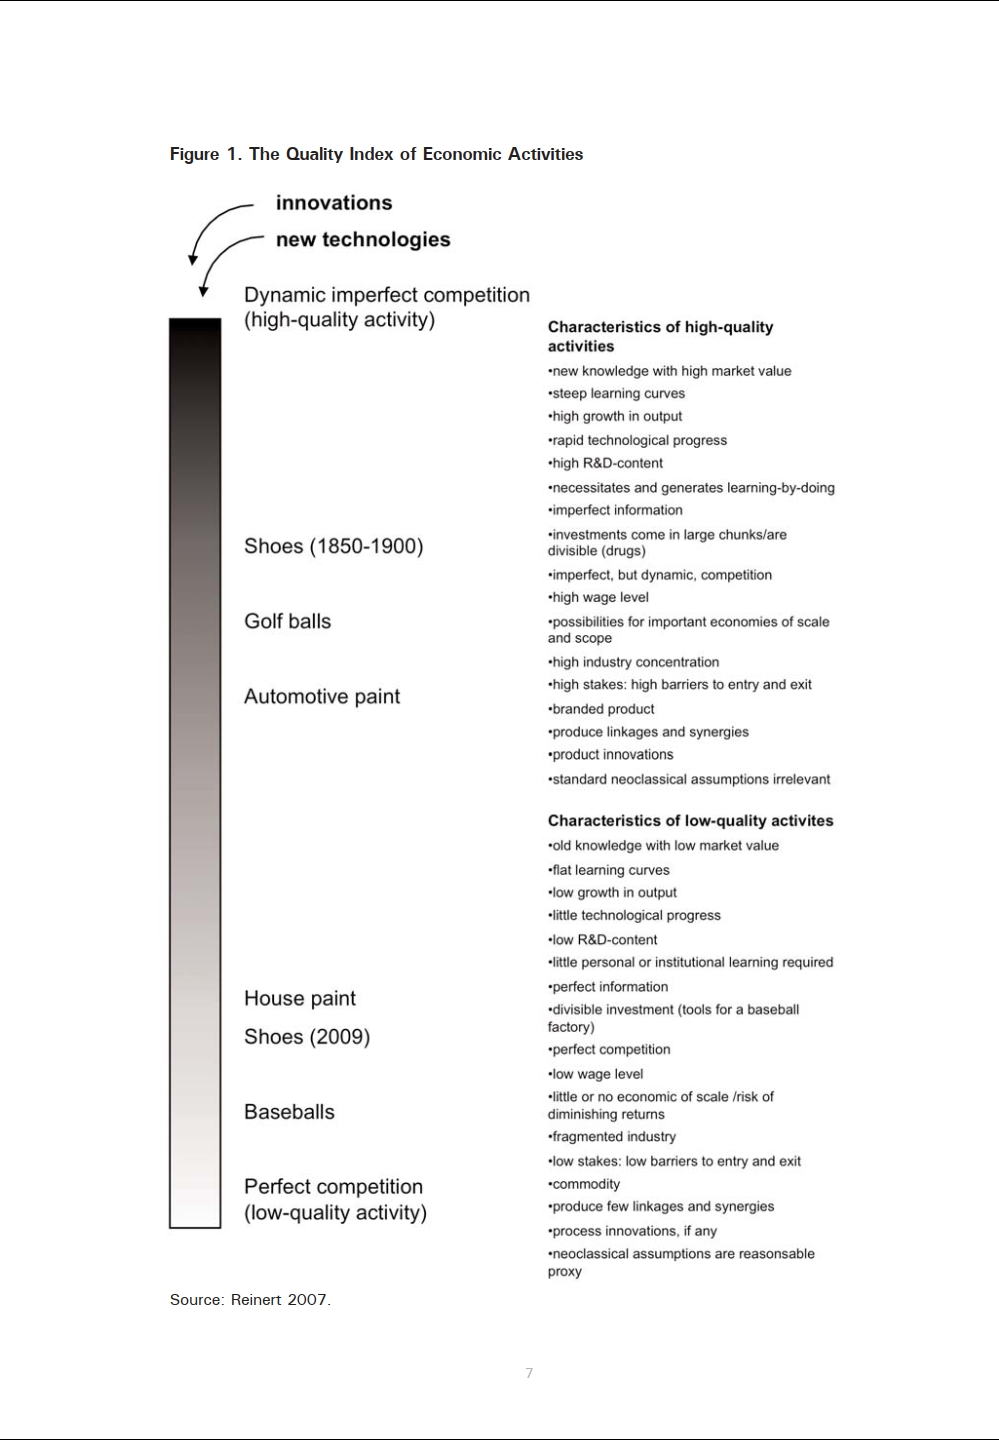
\includegraphics[width=0.5\linewidth]{../img/reinert.jpg}
	\end{figure}

\end{frame}

\begin{frame}{Protectionism}

\begin{columns}{}

\column{0.5\textwidth}

\begin{figure}[htpb]
	\centering
	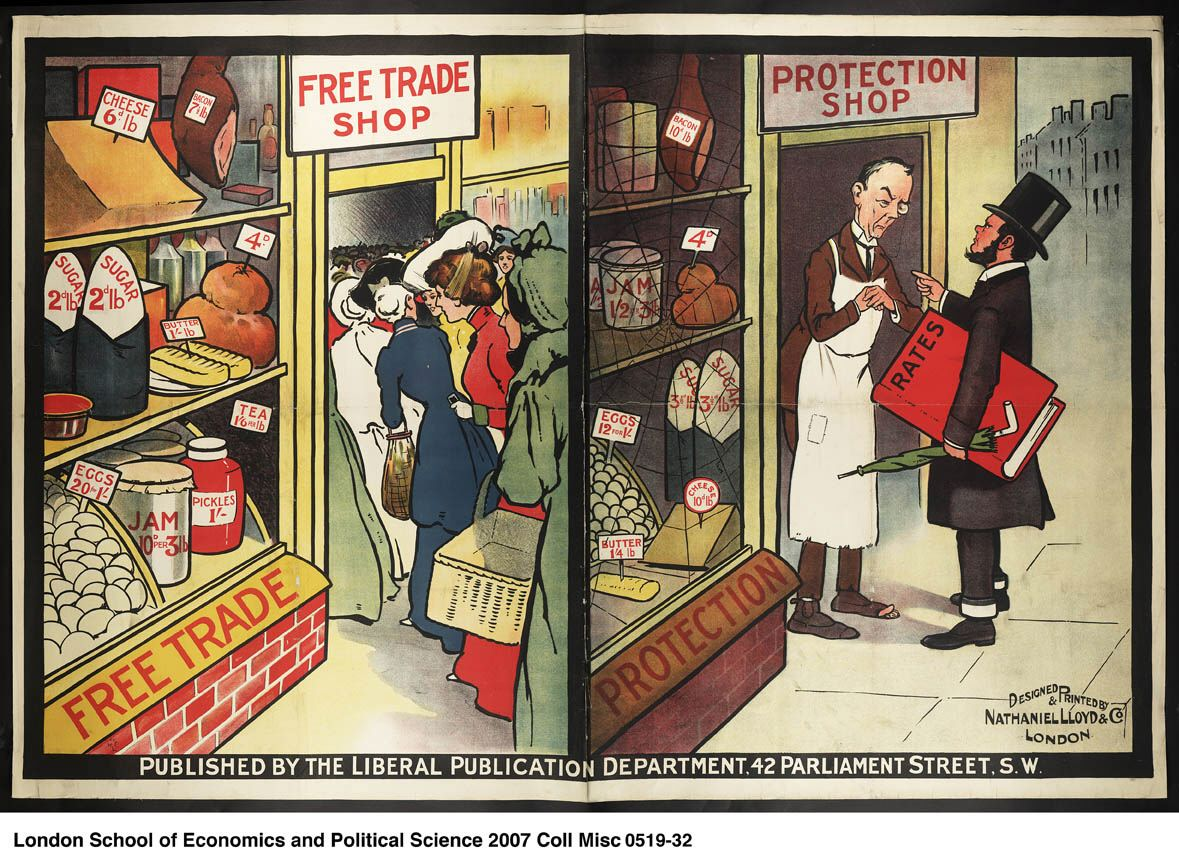
\includegraphics[width=1\textwidth]{../img/prodectionism.jpg}
\end{figure}

\column{0.5\textwidth}

\begin{figure}[htpb]
	\centering
	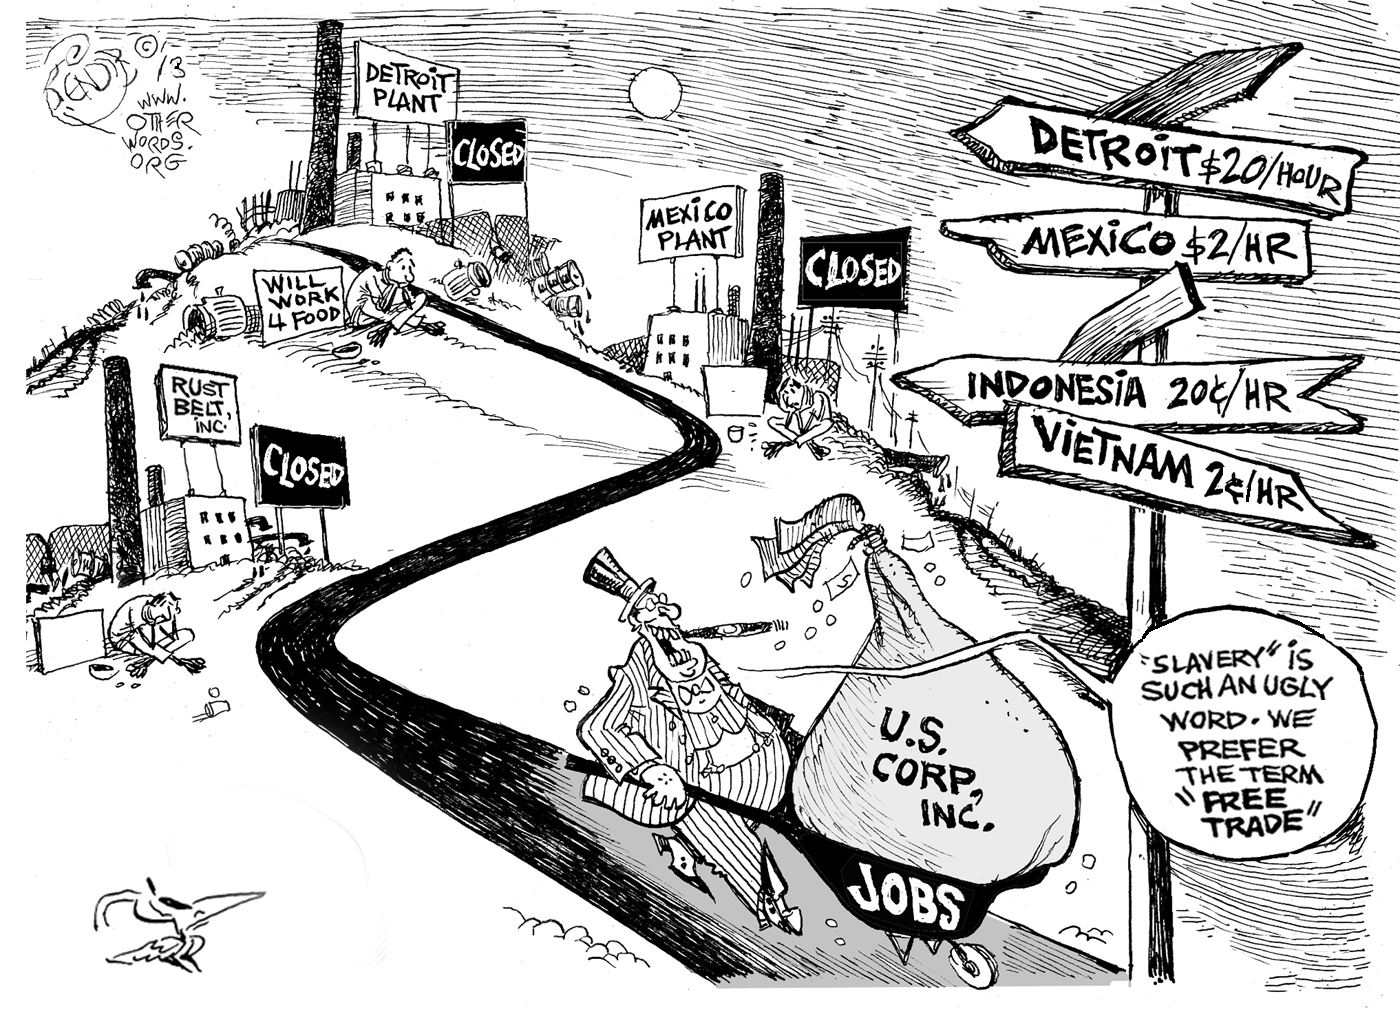
\includegraphics[width=1\linewidth]{../img/freetrade.jpeg}
\end{figure}

\end{columns}{}

\end{frame}

\section{Modern political economy} 

\begin{frame}{What is "modern political economy"}
	
\begin{itemize}
    \item The current state of the field \pause
    \item Reigning orthodoxy \pause
    \begin{itemize}
        \item Neo-classical + Keynesianism + Monetarism \pause
		% Monetarism MV === PQ, fight inflation
    \end{itemize}{}
    \item Reigning political movements \pause
    \begin{itemize}
        \item Neo-liberalism (US) \pause
        \item Populism? Protectionism? Anti-globalization...ism? Patriotism?
    \end{itemize}{}
\end{itemize}

\end{frame}{}

\begin{frame}{Dissidents} 
      \begin{itemize}
        \item Evolutionary economy \pause
        \item Marxists \pause
        \item Institutionalists 
    %   - Common features: 
    % 	- Relationship between capital, labor and state
    % 	- Studying change over time rather than static equilibrium
    % 	- Processes of circular and cumulative causation
    % 	- How resources are created/destroyed, not just allocated
    % 	- Role of politics (active/transformative)
      \end{itemize}
\end{frame}{}

\begin{frame}{More dissidents}
\begin{columns}[onlytextwidth]
\column{0.5\textwidth}
\begin{itemize}
    \item Feminism % How is the economy gendered?
    \item Environmentalism % Both have strong normative elements
    \item Behavioral economics
    %   - Behavioral/social psychology
    %   - Kahneman: Thinking fast and slow.
    % 	- Thaler & Sunstein: Nudge
    % 	- Importance of how a economic decisions are "framed"
    % 	- Consumer is NOT king - unless we crown him
\end{itemize}
\end{columns}
\end{frame}


\begin{frame}{More dissidents}
\begin{columns}[onlytextwidth]
\column{0.5\textwidth}
\begin{itemize}
    \item Feminism % How is the economy gendered?
    \item Environmentalism % Both have strong normative elements
    \item Behavioral economics
    %   - Behavioral/social psychology
    %   - Kahneman: Thinking fast and slow.
    % 	- Thaler & Sunstein: Nudge
    % 	- Importance of how a economic decisions are "framed"
    % 	- Consumer is NOT king - unless we crown him
    %   - Fast becoming part of the orthodox synthesis
\end{itemize}
\column{0.5\textwidth}
\begin{figure}
    \centering
    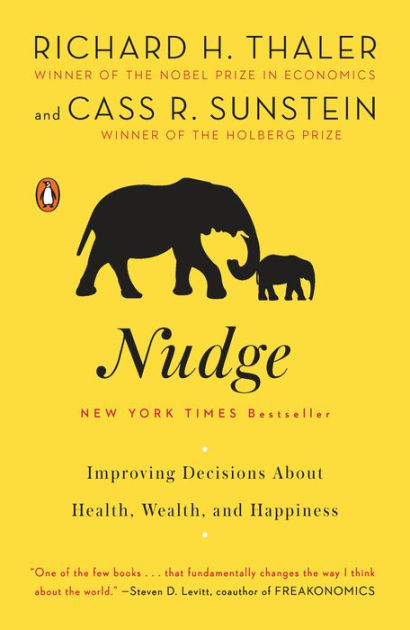
\includegraphics[width=0.9\textwidth]{../img/better nudge.jpg}
\end{figure}
\end{columns}
\end{frame}

\begin{frame}{"New" Themes in Political Economy} 
\begin{itemize}
    \item Nature % Environment
    \item Technology % Industry, work
    \item Society % Class, gender, ethnicity
    \item State
    % Themes that "modern political economists" grapple with
\end{itemize}{}
\end{frame}{}

\end{document}	
